Tässä luvussa esitetään perusteet ja tarvittavat tiedot hyväksymistestauksesta..

\section{Hyväksymistestauksen tarkoitus} \label{ch:08_hyvaksymistestauksen_tarkoitus}

  Hyväksymistestauksen tarkoituksena on varmistaa toteutettavan ohjelmiston vaatimusten toimivuus erityisesti käytännön tilanteissa siten, että voidaan varmistaa vastaako ohjelmisto loppukäyttäjän tarpeita.

  \begin{itemize}
    \item Painoarvo vaatimusmäärittelyssä
    \item mahdollisuus korjata virheet ennen julkaisua loppukäyttäjille
    \item keskitytään lähinnä toiminnallisiin ominaisuuksiin ja niiden toimivuuden varmistamiseen
    \item loppukäyttäjän tarpeet
    \item päästä päähän
    \item ohjelmistokehittäjien lisäksi myös sidosryhmät ja asiakkkat
    \item ab testaamisen mahdollisuus
    \item viimeinen vaihe testauksessa
    \item oikeat loppukäyttäjät tai käyttötapauksiin perustuva automaatio
    \item ei painoarvoa kosmeettisia virheissä tai kirjoitusvirheissä
    \item kehittäjien käsitys voi olla erilainen kuin loppukäyttäjien => kehittäjät pääsevät samalle sivulle
    \item prerequisites: vaatimukset, julkaisukelpoinen toteutus, vain kosmeettisia virheitä
    \item vaatimukset voi olla: liiketoimminnallisia käyttötapauksia, prosessivirtauskaavioita, vaatimusmäärittely
    \item toimiiko ohjelmisto loppukäyttäjän tarpeiden mukaisesti ja loppukäyttäjän näkökulmasta oikein
    \item toistuvalla hyväksymistestauksella varmistetaan, että ohjelma toteuttaa loppukäyttäjän tarpeet muutosten jälkeenkin
    \item hyväksymistestauksella saadaan katsaus ohjelmiston valmiudesta vaatimuksiin nähden
    \item ISTQB: Muodollista testaamista jossa käyttäjän tarpeet, vaatimukset ja liiketoimintaprosessit otetaan huomioon selvittäessä täyttääkö järjestelmä hyväksymisen kriteerit ja sallii käyttäjän, asiakkaiden tai muun autorisoidun tahon päättää hyväksytäänkö järjestelmä.
    \item teknisesti mustalaatikkotestausta
    \item hyväksymistestauksen testitapaukset tarkoituksenmukaisesti heijastavat suoraan loppukäyttäjien tarpeita
    \item käyttötapaus: 1) tilanne, 2) motivaatio, 3) haluttu lopputulos (esim. Kun tämä, niin haluan tätä, jotta saavutan tämän)
  \end{itemize}

\section{Hyväksymistestausvetoinen kehitys} \label{ch:08_hyvaksymistestausvetoinen_kehitys}

  Hyväksymistestausvetoisen kehityksen (englanniksi: ATDD, acceptance test driven development) tarkoituksena, kuten testausvetoisessakin kehityksessä on toteuttaa ohjelmistotuotannollinen prosessi testaaminen edellä.

  Tämä tarkoittaa käytännössä, sitä että ohjelmistokehittäjät laativat ohjelmiston vaatimusten ja suunnitelman mukaisia iteratiivisesti suoritettavia testitapauksia, ennen niitä käyttävän varsinaisen ohjelmakoodin toteuttamista.

  Hyväksymistestausvetoisessa kehityksessä luodaan ennen toteutusta tarvittavat ohjelmiston asiakasvaatimuksia palvelevat hyväksymistestit, joiden ohjelmiston on tarkoitus läpäistä.

  Tarvittavat ohjelmiston hyväksymistestit suoritetaan iteratiivisesti ohjelmistokehitysprosessin aikana, ja se tarkoittaa käytännössä jatkuvan integraation \ref{ch:07_jatkuva_integrointi} ottamista käyttöön ohjelmistokehityksessä.

  Hyväksysmistestausvetoinen kehitys on erittäin hyödyllinen ohjelmistokehityksessä käytetty menetelmä, sillä kehitysvaiheessa on aina tarkasti tiedossa vastaako ohjelmiston tila asiakasvaatimuksia ja kuinka hyvin se niiden täyttämisessä onnistuu.

  % TODO: Lisää kuva tähän ATDD:stä (kuten ch:07_testausvetoinen_kehitys)

  \begin{itemize}
    \item ketterä ohjelmistokehitysmenetelmä
    \item kuten tdd, mutta ennen ohjelmistokehityksen aloitusta asiakasvaatimukset kartoitetaan ja hyväksyttävyys määritetään
    \item ohjelmistokehitystä ohjaa vaatimukset ja loppukäyttäjien tarpeiden toteutuminen
    \item hyväksymistestit kirjoitetaan tdd:n mukaisesti ensin, ja ohjelmistokehitys noudattaa iteratiivisesti tdd:tä, vaikkakin hyväksymistestaus itsessään on perinteisesti vaatinut lähes valmista järjestelmää.
    \item hyväksymistestit pilkotaan pieniin hallittaviin kokonaisuuksiin, jolloin voidaan iteratiivisesti toteuttaa valmiiksi tietyn testitapauksen mukainen ominaisuus joka vastaa jotakin loppukäyttäjän tarvetta.
    \item testitapaus voi olla esimerkiksi käyttäjän tietojen muuttuminen varmistaminen, kuten tason läpäiseminen pelisovelluksessa, joka muuttaa käyttäjän edistystä.
    \item esimerkki käyttötapaus: as a user, I want to be able to unlock premium features by in-app purchase
    \item Perus workflow: 1) kirjoita vaatimus testitapauksen muotoon, 2) toteuta testitapaus ja ominaisuus, 3) refaktoroi ja iteroi takaisin 1 vaiheeseen tarvittaessa, 4) aja testitapaus ja validoi ominaisuuden toimivuus
    \item menetelmän tarkoituksena on onnistua vastaamaan loppukäyttäjän tarpeisiin tehokkaasti ja hyvin ottamalla tarpeet huomioon jo ennen toteutuksen aloittamista.
    \item menetelmän avulla myös luodaan ymmärrystä ohjelmistotuotteen valmiuden määritelmästä kun eri sidosryhmät pääsevät samalle aaltopituudelle.
    \item jatkuva testaaminen haluttujen ominaisuuksien toteutumisen validoimiselle menetelmän jokaisen iteraation koontiversiossa.
    \item hyväksymistestausvetoinen kehitys lainaa samoja perusperiaatteita testausvetoisesta kehityksestä, mutta keskittyy käyttötapauksien muodossa validoitavien haluttujen ominaisuuksien toteutumista.
  \end{itemize}

\section{Robot Framework} \label{ch:08_robot_framework}

  Robot framework on geneerinen avoimen lähdekoodin testausalusta hyväksymistestaukseen, hyväksymistestausvetoiseen kehitykseen ja robotisten prosessien automaatioon.

  \begin{figure}[H]
    \centering
    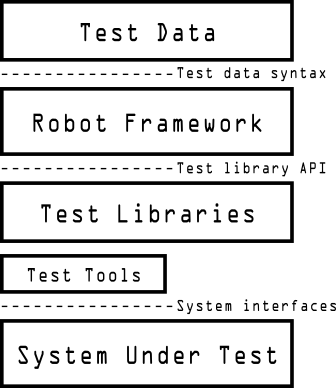
\includegraphics[width=0.4\textwidth]{assets/robot-architecture.png}
    \caption{Robot framework alustan arkkitehtuuri}
    \label{fig:robot-architecture}
  \end{figure}

  \begin{itemize}
    \item Helposti ymmärrettävä, luettava ja selkeä avainsanaperustainen syntaksi
    \item Etuna helposti lähestyttävyys. Helppo asentaa, ymmärtää ja ottaa käyttöön.
    \item Testikehystä voi helppouden ja avainsanaperustaisuuden vuoksi käyttää muutkin kuin sovelluskehittäjät.
    \item Tuki ulkoisille kirjastoille ja useita käyttövalmiita ulkoisia kirjastoja
    \item Tukee muuttujia testitapauksissa, joilla voi lisätä hieman kompleksisuutta testitapauksiin
    \item Tukee dataperustaisia testitapauksia, joille annetaan eri syötteitä sisältävää testidataa
    \item Testitapauksia voidaan ryhmitellä tageillä.
    \item Kattavat ja selkeät testiraportit ajetuille testitapauksille.
    \item Heikkoutena tuen puuttuminen ohjelmointikieliperustaisissa testikehyksissä löytyville kontrollirakenteille, joita esiintyy esimerkiksi yksikkötestaukseen tarkoitetuissa testikehyksissä.
  \end{itemize}

\section{Testitapauksien määrittäminen} \label{ch:08_testitapauksien_maarittaminen}

  \begin{itemize}
    \item Testitapaus on testiautomaation näkökulmasta, määritelty toimenpiteiden, ehtojen ja muuttujien joukko, joka suorittamalla voidaan verifioida ominaisuus tai toiminnallisuus ohjelmistosta.
    \item Testisuite tai testikokoelma on samaan kontekstiin kuuluvista testitapauksista muodostettu joukko.
    \item Testitapaukset kirjoitetaan hyväksymistestauksen mukaisesti käyttötapauksien muodossa.
    \item Testiformaatti: 1) Oletetaan tämä ja tätä (setup) => 2) Kun tämä tapahtuu (trigger) => 3) Niin tämä seuraa (verification) (todo: tee tästä kuva)
    \item Yleisiä tavoitteita: yksinkertaisuus, läpinäkyvyys, käyttäjätietoisuus, epätoistuvuus, olettamattomuus, kattavuus, tunnistettavuus, jälkensä puhdistava, toistettava, syvyyttömyys, atomisuus.
    \item Taulukon/listan muodossa esimerkkejä käyttöliittymien testitapauksista.
    \item Robot framework: avainsana, käyttäytyminen tai data-pohjainen kirjoitustyyli testitapauksille
    % \item <todo: lisää kuva/koodi esimerkkitestitapauksessa robot frameworkillä>
    \item https://github.com/robotframework/HowToWriteGoodTestCases/blob/master/HowToWriteGoodTestCases.rst
  \end{itemize}

\section{Web-käyttöliittymien erityispiirteet} \label{ch:08_webkayttoliittymien_erityispiirteet}

  Web-käyttöliittymillä on myös omia erityispiirteitä, jotka vaikuttavat testitapauksien laatimiseen.

  \begin{itemize}
    \item Käyttöliittymä ja DOM
    \item Hosting
    \item Näyttöresoluutiot
    \item Navigointi
    \item Syötteet
    \item Syntaksi
    \item Selainasetukset
    \item Moniselaimellinen testaus
    \item Päätteetön testaus
    \item Selenium
  \end{itemize}

\section{Priorisointiongelma} \label{ch:08_priorisointiongelma}

  Testitapauksien priorisointi on kustannussyistä tai resurssien optimoinnin kannalta erittäin tärkeää.
  Ohjelmistotestauksessa on hyvä tiedostaa, että ohjelmistotuotetta ei usein voida testata täydellisesti, joka nostaa esiin tarpeen tärkeimpien testitapauksien löytämisestä.
  Testitapauksia voidaan priorisoida monella tavalla, joihin tämä diplomityö tuo yhden uudenlaisen painottua verkkoa hyödyntävän lähestymistavan.

  \begin{itemize}
    \item Painotetun verkon hyödyntäminen
    \item Muut priorisointitavat
  \end{itemize}